\documentclass[a4paper]{article} 
\usepackage{texthanglist}
\usepackage{verbatim} 
\usepackage{multicol}
\usepackage{changepage}
\usepackage{float}
\usepackage{grffile}
\usepackage{graphicx}
\usepackage{amssymb}
\usepackage{fontspec}
\usepackage{fancyhdr}
\usepackage{multicol}
\usepackage{calc}
\usepackage[margin=1cm,includeheadfoot]{geometry}
\usepackage{eso-pic}
\pagestyle{plain}\pagestyle{fancy}
\renewcommand{\headrulewidth}{0.4pt} \renewcommand{\footrulewidth}{0.4pt}

\begin{document} 
\pagestyle{plain} 
\font\spanParagraphContinuationscrSectioncolumnsscrBookscrBody="Times New Roman" at 12pt
\font\VerseNumberParagraphContinuationscrSectioncolumnsscrBookscrBody="Times New Roman" at 6pt
\font\ParagraphContinuationscrSectioncolumnsscrBookscrBody="Times New Roman" at 12pt
\font\spanreferenceafterpictureCaptionpictureColumnParagraphscrSectioncolumnsscrBookscrBody="Times New Roman" at 12pt
\font\spanreferencebeforepictureCaptionpictureColumnParagraphscrSectioncolumnsscrBookscrBody="Times New Roman" at 12pt
\font\spanpictureCaptionpictureColumnParagraphscrSectioncolumnsscrBookscrBody="Times New Roman" at 12pt
\font\pictureCaptionpictureColumnParagraphscrSectioncolumnsscrBookscrBody="Times New Roman" at 12pt
\font\picturepictureColumnParagraphscrSectioncolumnsscrBookscrBody="Times New Roman" at 12pt
\font\pictureColumnParagraphscrSectioncolumnsscrBookscrBody="Times New Roman" at 12pt
\font\spanreferenceafterpictureCaptionpicturePageParagraphscrSectioncolumnsscrBookscrBody="Times New Roman" at 12pt
\font\spanreferencebeforepictureCaptionpicturePageParagraphscrSectioncolumnsscrBookscrBody="Times New Roman" at 12pt
\font\spanpictureCaptionpicturePageParagraphscrSectioncolumnsscrBookscrBody="Times New Roman" at 12pt
\font\pictureCaptionpicturePageParagraphscrSectioncolumnsscrBookscrBody="Times New Roman" at 12pt
\font\picturepicturePageParagraphscrSectioncolumnsscrBookscrBody="Times New Roman" at 12pt
\font\picturePageParagraphscrSectioncolumnsscrBookscrBody="Times New Roman" at 12pt
\font\SeeInGlossaryParagraphscrSectioncolumnsscrBookscrBody="Times New Roman":color=0000ff at 12pt
\font\spanLinecscrSectioncolumnsscrBookscrBody="Times New Roman" at 12pt
\font\LinecscrSectioncolumnsscrBookscrBody="Times New Roman" at 12pt
\font\SeeInGlossaryLinebscrSectioncolumnsscrBookscrBody="Times New Roman":color=0000ff at 12pt
\font\spanLinebscrSectioncolumnsscrBookscrBody="Times New Roman" at 12pt
\font\VerseNumberLinebscrSectioncolumnsscrBookscrBody="Times New Roman" at 6pt
\font\LinebscrSectioncolumnsscrBookscrBody="Times New Roman" at 12pt
\font\spanNoteGeneralParagraphParagraphscrSectioncolumnsscrBookscrBody="Times New Roman" at 12pt
\font\AlternateReadingNoteGeneralParagraphParagraphscrSectioncolumnsscrBookscrBody="Times New Roman/I" at 12pt
\font\NoteTargetReferenceNoteGeneralParagraphParagraphscrSectioncolumnsscrBookscrBody="Times New Roman/B" at 12pt
\font\NoteGeneralParagraphParagraphscrSectioncolumnsscrBookscrBody="Times New Roman" at 12pt
\font\spanParagraphscrSectioncolumnsscrBookscrBody="Times New Roman" at 12pt
\font\VerseNumberParagraphscrSectioncolumnsscrBookscrBody="Times New Roman" at 6pt
\font\ChapterNumberParagraphscrSectioncolumnsscrBookscrBody="Times New Roman/B" at 18pt
\font\ParagraphscrSectioncolumnsscrBookscrBody="Times New Roman" at 12pt
\font\spanParallelPassageReferencescrSectioncolumnsscrBookscrBody="Times New Roman/I" at 12pt
\font\ParallelPassageReferencescrSectioncolumnsscrBookscrBody="Times New Roman/I" at 12pt
\font\spanSectionHeadscrSectioncolumnsscrBookscrBody="Times New Roman/B" at 12pt
\font\SectionHeadscrSectioncolumnsscrBookscrBody="Times New Roman/B" at 12pt
\font\scrSectioncolumnsscrBookscrBody="Times New Roman" at 12pt
\font\columnsscrBookscrBody="Times New Roman" at 12pt
\font\spanTitleMainscrBookscrBody="Times New Roman/B" at 18pt
\font\TitleSecondaryTitleMainscrBookscrBody="Times New Roman/BI" at 16pt
\font\TitleMainscrBookscrBody="Times New Roman/B" at 18pt
\font\scrBookCodescrBookscrBody="Times New Roman/BI" at 12pt
\font\scrBookNamescrBookscrBody="Times New Roman/I" at 12pt
\font\scrBookscrBody="Times New Roman" at 12pt
\font\imgpicturedivpictureLeft="Times New Roman" at 12pt
\font\picturepictureRight="Times New Roman" at 12pt
\font\spanzhCN="SimSun" at 12pt
\font\divzhCN="SimSun" at 12pt
\font\spanur="Scheherazade Graphite Alpha" at 12pt
\font\divur="Scheherazade Graphite Alpha" at 12pt
\font\spanurxind="Times New Roman" at 12pt
\font\divurxind="Times New Roman" at 12pt
\font\spantr="Charis SIL" at 12pt
\font\divtr="Charis SIL" at 12pt
\font\spantrfonipa="Doulos SIL" at 12pt
\font\divtrfonipa="Doulos SIL" at 12pt
\font\spantrfonipaxemic="Times New Roman" at 12pt
\font\divtrfonipaxemic="Times New Roman" at 12pt
\font\spantpi="Times New Roman" at 12pt
\font\divtpi="Times New Roman" at 12pt
\font\spante="Gautami" at 12pt
\font\divte="Gautami" at 12pt
\font\spanseh="Doulos SIL" at 12pt
\font\divseh="Doulos SIL" at 12pt
\font\spanru="Times New Roman" at 12pt
\font\divru="Times New Roman" at 12pt
\font\spanqaaxcam="Times New Roman" at 12pt
\font\divqaaxcam="Times New Roman" at 12pt
\font\spanpt="Times New Roman" at 12pt
\font\divpt="Times New Roman" at 12pt
\font\spannko="Charis SIL" at 12pt
\font\divnko="Charis SIL" at 12pt
\font\spanmy="Padauk" at 12pt
\font\divmy="Padauk" at 12pt
\font\spanko="Gulim" at 12pt
\font\divko="Gulim" at 12pt
\font\spanid="Times New Roman" at 12pt
\font\divid="Times New Roman" at 12pt
\font\spanhi="Arial Unicode MS" at 12pt
\font\divhi="Arial Unicode MS" at 12pt
\font\spanhe="Ezra SIL" at 12pt
\font\divhe="Ezra SIL" at 12pt
\font\spanhbo="Ezra SIL" at 12pt
\font\divhbo="Ezra SIL" at 12pt
\font\spangrc="Galatia SIL" at 12pt
\font\divgrc="Galatia SIL" at 12pt
\font\spanggoTeluIN="Gautami" at 12pt
\font\divggoTeluIN="Gautami" at 12pt
\font\spanggofonipaxemic="Tahoma" at 12pt
\font\divggofonipaxemic="Tahoma" at 12pt
\font\spanfr="Times New Roman" at 12pt
\font\divfr="Times New Roman" at 12pt
\font\spanfa="Times New Roman" at 12pt
\font\divfa="Times New Roman" at 12pt
\font\spanes="Times New Roman" at 12pt
\font\dives="Times New Roman" at 12pt
\font\spanen="Times New Roman" at 12pt
\font\diven="Times New Roman" at 12pt
\font\spanenQaaaxtest="Charis SIL Compact" at 12pt
\font\divenQaaaxtest="Charis SIL Compact" at 12pt
\font\spanenfonipa="Doulos SIL" at 12pt
\font\divenfonipa="Doulos SIL" at 12pt
\font\spande="Times New Roman" at 12pt
\font\divde="Times New Roman" at 12pt
\font\spanbzh="Charis SIL" at 12pt
\font\divbzh="Charis SIL" at 12pt
\font\spanbzhfonipa="Doulos SIL" at 12pt
\font\divbzhfonipa="Doulos SIL" at 12pt
\font\spanbss="Charis SIL" at 12pt
\font\divbss="Charis SIL" at 12pt
\font\spanbssxako="Charis SIL Compact" at 12pt
\font\divbssxako="Charis SIL Compact" at 12pt
\font\spanbssfonipa="Charis SIL Compact" at 12pt
\font\divbssfonipa="Charis SIL Compact" at 12pt
\color{black} 
\AddToShipoutPicture*{% 
\put(0,0){\rule{\paperwidth}{\paperheight}}{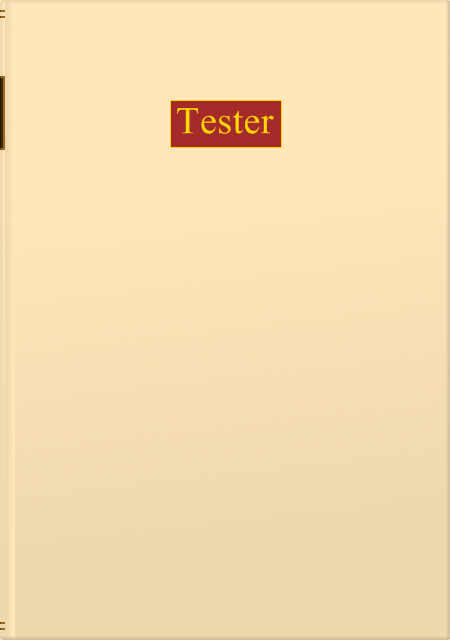
\includegraphics[width=\paperwidth, height=\paperheight]{cover.png}}% 
} 
\thispagestyle{empty} 
\font\CoverPageHeading="Times New Roman/B":color=000000 at 22pt 
\vskip 60pt 
\begin{center} 
\CoverPageHeading{Nkonya Sample} 
\end{center} 
\newpage 
\newpage 
\thispagestyle{empty} 
\mbox{} 

\pagestyle{fancy} 
\begin{comment}

\scrBookNamescrBookscrBody{
 \section{Mateo} }\end{comment}
  \begin{comment}
\scrBookCodescrBookscrBody{MAT}\end{comment}
  \begin{adjustwidth}{36pt}{0pt}{12pt}{0pt}\begin{center}\begin{adjustwidth}{0pt}{0pt}{2pt}{0pt}\begin{center}

\TitleSecondaryTitleMainscrBookscrBody{Asʋn Wankláán Ánɩ́ }\end{center}\end{adjustwidth} 

\spanTitleMainscrBookscrBody{Mateo }\begin{adjustwidth}{0pt}{0pt}{2pt}{0pt}\begin{center}

\TitleSecondaryTitleMainscrBookscrBody{Lɔ́wanlɩ́n }\end{center}\end{adjustwidth} 
\end{center}\end{adjustwidth} \setlength{\columnsep}{12pt} 
\setlength\columnseprule{0.4pt} 
\begin{multicols}{2}{\raggedright} \begin{adjustwidth}{0pt}{0pt}{0pt}{0pt}\begin{center}
\spanSectionHeadscrSectioncolumnsscrBookscrBody{Bɔhɔ Yesu Fɛ́ Owíe Yerusalem }\end{center}\end{adjustwidth} 
\begin{adjustwidth}{0pt}{0pt}{4pt}{0pt}\begin{center}
\spanParallelPassageReferencescrSectioncolumnsscrBookscrBody{(Marko 11:1-11; Luka 19:28-40; Yohane 12:12-19) }\end{center}\end{adjustwidth} 

\leftmargin 0pt{\ChapterNumberParagraphscrSectioncolumnsscrBookscrBody{21}}\leftmargin 0pt{\VerseNumberParagraphscrSectioncolumnsscrBookscrBody{$^{1-2}$}} \spanParagraphscrSectioncolumnsscrBookscrBody{Brɛ́á Yesu mʋa mʋ akasɩ́pʋ́ bɛbɛ́ɛn Yerusalem wúlu, bɛta Betfage wúlu ánɩ́ ɩbʋ Nfɔ-nyíbʋ}   \footnote {21:1 Nfɔ-nyíbʋ igyi obubwí kʋá ɩbʋ mantáa Yerusalem, bʋtɛtɩ́ mʋ́ Olifbʋ.} \spanParagraphscrSectioncolumnsscrBookscrBody{ámʋ asɩ wie tá á, ɔlɔwa mʋ akasɩ́pʋ́ abanyɔ́ gyankpá. Ɔlɛbláa amʋ́ ɔbɛ́ɛ, $“$Mlɩyɔ wúlu anfɩ́ ɩda mlɩ ansɩ́tɔ́ ánfɩsʋ. Nɩ́ mlowíé wúlu amʋ ɔnɔ́ á, mlówun afrímú tsɩ́hɛ́ ɔkʋá ɔda ɔfɛ́tɔ́, mʋ bi lɩ́ɩ́ mʋ wá. Mlɩsankɩ mʋ, amlɩkpa amʋ́ ba mɩ. }\leftmargin 0pt{\VerseNumberParagraphscrSectioncolumnsscrBookscrBody{$^{3}$}} \spanParagraphscrSectioncolumnsscrBookscrBody{Nɩ́ ɔkʋ ɔfɩ́tɛ́ mlɩ asʋankʋ á, mlɩbla mʋ mlɩaa, $‘$Anɩ Wíe dɛ́ amʋ́ hián.$’$ Ɩnʋnʋ ɔbɛ́ha mlɔ́pʋ amʋ́ ba mɩ.$”$ }

\leftmargin 0pt{\VerseNumberParagraphscrSectioncolumnsscrBookscrBody{$^{4}$}} \spanParagraphscrSectioncolumnsscrBookscrBody{Ɩ́nɩ lɛ́ha Bulu asʋ́n ámʋ́ʋ́ ɔlɛblɩ́ tsʋn mʋ ɔnɔ́sʋ́ ɔtɔɩ́pʋ́sʋ ámʋ lɛ́ba mʋ́tɔ́. Ɔbɛ́ɛ, }
\begin{adjustwidth}{0pt}{0pt}{0pt}{0pt}{\raggedright} 
\leftmargin 0pt{\VerseNumberLinebscrSectioncolumnsscrBookscrBody{$^{5}$}} \spanLinebscrSectioncolumnsscrBookscrBody{$“$Mlɩbla }\SeeInGlossaryLinebscrSectioncolumnsscrBookscrBody{Sionfɔ} \spanLinebscrSectioncolumnsscrBookscrBody{mlɩaa, } \end{adjustwidth} 
\begin{adjustwidth}{0pt}{0pt}{0pt}{0pt}{\raggedright} 
\spanLinecscrSectioncolumnsscrBookscrBody{Mlɩkɩ, mlɩ Wíe ɔbá mlɩ wá. } \end{adjustwidth} 
\begin{adjustwidth}{0pt}{0pt}{0pt}{0pt}{\raggedright} 
\spanLinebscrSectioncolumnsscrBookscrBody{Ololwií, ɔdɩn afrímúsʋ́. } \end{adjustwidth} 
\begin{adjustwidth}{0pt}{0pt}{0pt}{0pt}{\raggedright} 
\spanLinecscrSectioncolumnsscrBookscrBody{Ɔdɩn afrímú ibí yínhɛ́sʋ́ ɔbá.$”$ } \end{adjustwidth} 

\leftmargin 0pt{\VerseNumberParagraphscrSectioncolumnsscrBookscrBody{$^{6}$}} \spanParagraphscrSectioncolumnsscrBookscrBody{Yesu akasɩ́pʋ́ abanyɔ́ ámʋ bɔyɔ́bwɛ alɩ ámʋ́ʋ́ Yesu lɛ́bláa amʋ́ ámʋ. }\leftmargin 0pt{\VerseNumberParagraphscrSectioncolumnsscrBookscrBody{$^{7}$}} \spanParagraphscrSectioncolumnsscrBookscrBody{Bɛkpa afrímú mʋa mʋ bi ámʋ ba, bɛyaɩ́ amʋ́ atati dɩ́nká amʋ́sʋ́, ɔlɔdʋ bian mʋsʋ. }\leftmargin 0pt{\VerseNumberParagraphscrSectioncolumnsscrBookscrBody{$^{8}$}} \spanParagraphscrSectioncolumnsscrBookscrBody{Ɔdɔm kpɔnkpɔɔnkpɔntɩ bɛyaɩ́ amʋ́ atati tswɩ ɔkpatɔ, akʋ ɛ́ bebiabía afɩtáa bunbun ɔkpa ámʋtɔ. }\leftmargin 0pt{\VerseNumberParagraphscrSectioncolumnsscrBookscrBody{$^{9}$}} \spanParagraphscrSectioncolumnsscrBookscrBody{Ɔdɔm amʋ́ʋ́ bʋgya Yesu nkpá mʋ́a ɔma amʋ bɔsʋrá okitikíti bɛɛ, $“$} \SeeInGlossaryParagraphscrSectioncolumnsscrBookscrBody{Hosiána} \spanParagraphscrSectioncolumnsscrBookscrBody{há Dawid mʋ na ámʋ! Bulu oyúla owíe anfɩ ɔbá mʋ dátɔ́ ánfɩ! Hosiána bʋ ɔsʋ́sʋ́ʋ́sʋ́!$”$ }

\leftmargin 0pt{\VerseNumberParagraphscrSectioncolumnsscrBookscrBody{$^{10}$}} \spanParagraphscrSectioncolumnsscrBookscrBody{Brɛ́á Yesu lówie Yerusalem a, wúlu amʋtɔ fɛ́ɛ́ lɛda kpokiti, bʋdɛfɩtɛ́ bɛɛ, $“$Ma gyí ɔhá ánfɩ?$”$ }

\leftmargin 0pt{\VerseNumberParagraphscrSectioncolumnsscrBookscrBody{$^{11}$}} \spanParagraphscrSectioncolumnsscrBookscrBody{Ɔdɔm amʋ́ʋ́ bʋbuo mʋ amʋ bɛlɛ mʋ́ ɔnɔ́ bɛɛ, $“$Ɔ́nɩ gyí Yesu, Bulu ɔnɔ́sʋ́ ɔtɔɩ́pʋ́ amʋ́ʋ́ otsú Nasaret wúluá ɩbʋ Galilea ɔmátɔ́ ámʋ nɩ.$”$ }
 {\raggedright} \begin{adjustwidth}{0pt}{0pt}{0pt}{0pt}\begin{center}
\spanSectionHeadscrSectioncolumnsscrBookscrBody{Yesu Bulu Ɔtswɛ́kpa Yɔ }\end{center}\end{adjustwidth} 
\begin{adjustwidth}{0pt}{0pt}{4pt}{0pt}\begin{center}
\spanParallelPassageReferencescrSectioncolumnsscrBookscrBody{(Marko 11:15-19; Luka 19:45-48; Yohane 2:13-22) }\end{center}\end{adjustwidth} 

\leftmargin 0pt{\VerseNumberParagraphscrSectioncolumnsscrBookscrBody{$^{12}$}} \spanParagraphscrSectioncolumnsscrBookscrBody{Mʋ́ʋ́ Yesu lɔ́yɔ }\SeeInGlossaryParagraphscrSectioncolumnsscrBookscrBody{Bulu ɔtswɛ́kpa} \spanParagraphscrSectioncolumnsscrBookscrBody{wunsɩnɛ́sʋ́ ɩnʋ, yégya atɔ́ afɛpʋ́ pʋ́ atɔ́ ahɔ́pʋ fɛ́ɛ́ dalɩ. Olowuwúta kɔ́ba atsɛ́pʋ mpʋ́nʋ́ dá, súnsúnki abrɔ́dʋma afɛpʋ́ ɛ́ mbíá dá. }\leftmargin 0pt{\VerseNumberParagraphscrSectioncolumnsscrBookscrBody{$^{13}$}} \spanParagraphscrSectioncolumnsscrBookscrBody{Ɔlɛbláa amʋ́ ɔbɛ́ɛ, $“$Bɔwanlɩ́n wá Bulu asʋ́n ámʋtɔ bɛɛ, $‘$Bɛ́tɩ mɩ́ ɔtswɛ́kpa bɛɛ, mpáɩ ɔbɔkpá.$’$ Támɛ mlɩlapʋ́ ɩnʋ mlí awikplu ɔŋaínkpá.$”$ }

\leftmargin 0pt{\VerseNumberParagraphscrSectioncolumnsscrBookscrBody{$^{14}$}} \spanParagraphscrSectioncolumnsscrBookscrBody{Ansibi abwiepʋ́ pʋ́ abubúpʋ akʋ bɛba mʋ wá Bulu ɔtswɛ́kpa wunsɩnɛ́sʋ́ ɩnʋ, ɔlɛtsa amʋ́ ɩlɔ. }\leftmargin 0pt{\VerseNumberParagraphscrSectioncolumnsscrBookscrBody{$^{15}$}} \spanParagraphscrSectioncolumnsscrBookscrBody{Brɛ́á Bulu }\SeeInGlossaryParagraphscrSectioncolumnsscrBookscrBody{igyí} \spanParagraphscrSectioncolumnsscrBookscrBody{ahapʋ́ dɛhɛn pʋ́ Mose mbla asunápʋ́ amʋ bowun ofúla ánɩ́ Yesu dɛ́bwɛ, pʋ́ alɩá nyebí bʋdɛkplʋ́n Bulu ɔtswɛ́kpa wunsɩnɛ́sʋ́ ɩnʋ bɛɛ, $“$Hosiána há Dawid mʋ na ámʋ!$”$ a, ɔblɔ́ lɛkɩtá amʋ́. }\leftmargin 0pt{\VerseNumberParagraphscrSectioncolumnsscrBookscrBody{$^{16}$}} \spanParagraphscrSectioncolumnsscrBookscrBody{Mʋ́ sʋ bɛfɩtɛ́ Yesu bɛɛ, $“$Fʋmedénu asʋ́n ánɩ́ nyebí ánfɩ bʋdɛblɩ́?$”$ }

\spanParagraphscrSectioncolumnsscrBookscrBody{Yesu lɛ́lɛ mʋ́ ɔnɔ́ ɔbɛ́ɛ, $“$Ndenu. Mlɩmɔ́kʋ́kla asʋ́n ánɩ́ Bulu asʋ́n wanlɩ́nhɛ́ amʋ lɛ́blɩ́? Ɔbɛ́ɛ, $‘$Fasúná nyebí pʋ́ amʋ́á bʋmɔkʋ́tɩn nyɔ́pʋ alɩá bʋkánfʋ fʋ́.$’$ $”$ }

\leftmargin 0pt{\VerseNumberParagraphscrSectioncolumnsscrBookscrBody{$^{17}$}} \spanParagraphscrSectioncolumnsscrBookscrBody{Yesu lɛ́dalɩ wúlu amʋtɔ sí amʋ́ yɔ́ Betania. Ɩnʋ́ ɔlɛdɩ ɛkɛ ámʋ nɩ. }
 {\raggedright} \begin{adjustwidth}{0pt}{0pt}{0pt}{0pt}\begin{center}
\spanSectionHeadscrSectioncolumnsscrBookscrBody{Pɔntɔ Oyí Lwɩɩ́ }\end{center}\end{adjustwidth} 
\begin{adjustwidth}{0pt}{0pt}{4pt}{0pt}\begin{center}
\spanParallelPassageReferencescrSectioncolumnsscrBookscrBody{(Marko 11:12-14, 20-24) }\end{center}\end{adjustwidth} 

\leftmargin 0pt{\VerseNumberParagraphscrSectioncolumnsscrBookscrBody{$^{18}$}} \spanParagraphscrSectioncolumnsscrBookscrBody{Ɔyɩ kɛhɛ nyankɩ, brɛ́á Yesu léyinkí ɔbá Yerusalem a, akʋ́n dɛ mʋ. }\leftmargin 0pt{\VerseNumberParagraphscrSectioncolumnsscrBookscrBody{$^{19}$}} \spanParagraphscrSectioncolumnsscrBookscrBody{Mʋ́ sʋ brɛ́á olowun pɔntɔ kʋá ɩlɩɩ́ mantáa ɔkpa á, ɔlɛbaɩ́ yɔ́ mʋ́ asɩ. Ɔlɔyɔ á, omowun abí kʋkʋ mʋ́tɔ́, afɩtáa sɔ́ɔ́n bʋ mʋ́sʋ́. Ɩnʋ ɔlɛbláa pɔntɔ ámʋ ɔbɛ́ɛ, $“$Tsú ndɛ fʋmɛ́ɛtrá swie abí ɛkɛkɛɛkɛ!$”$ Ɩnʋnʋ oyí ámʋ lówu. }

\leftmargin 0pt{\VerseNumberParagraphscrSectioncolumnsscrBookscrBody{$^{20}$}} \spanParagraphscrSectioncolumnsscrBookscrBody{Mʋ akasɩ́pʋ́ amʋ bowun alɩá oyí ámʋ labwɛ́ á, ɔnɔ́ lobwie amʋ́. Mʋ́ sʋ bɛfɩtɛ́ bɛɛ $“$Ntogyi sʋ́ oyí ánfɩ lawú ɔtsáwʋlɛ pɛ́ alɩ?$”$ }

\leftmargin 0pt{\VerseNumberParagraphscrSectioncolumnsscrBookscrBody{$^{21}$}} \spanParagraphscrSectioncolumnsscrBookscrBody{Yesu lɛ́bláa amʋ́ ɔbɛ́ɛ, $“$Ɔnɔkwalɩ ndɛ mlɩ bláa. Nɩ́ mlɔhɔ Bulu gyi, mlɩmégyi nwɛ́ɛn a, mlɛ́talɩ́ bwɛ́ ɩtɔ́ ánfɩ nabwɛ́ oyí ánfɩ pʋ́ mʋ́á ɩdʋn mʋ́. Mlɛ́talɩ́ bláa ɩbʋ ánfɩ mlɩaa, $‘$Puli yowie ɔpʋtɔ.$’$ Ibópulí yɔ́. }\leftmargin 0pt{\VerseNumberParagraphscrSectioncolumnsscrBookscrBody{$^{22}$}} \spanParagraphscrSectioncolumnsscrBookscrBody{Nɩ́ mlɔhɔ Bulu gyi, mlɔkʋ́lɩ́ mʋ tógyítɔ́ á, mlɩ ɩbɩ bɛ́da mʋ́.$”$ }
 {\raggedright} \begin{adjustwidth}{0pt}{0pt}{0pt}{0pt}\begin{center}
\spanSectionHeadscrSectioncolumnsscrBookscrBody{Yesu Túmi Ɩwɩ Asʋn Fɩtɛ́hɛ́ }\end{center}\end{adjustwidth} 
\begin{adjustwidth}{0pt}{0pt}{4pt}{0pt}\begin{center}
\spanParallelPassageReferencescrSectioncolumnsscrBookscrBody{(Marko 11:27-33; Luka 20:1-8) }\end{center}\end{adjustwidth} 

\leftmargin 0pt{\VerseNumberParagraphscrSectioncolumnsscrBookscrBody{$^{23}$}} \spanParagraphscrSectioncolumnsscrBookscrBody{Yesu léyinkí bowie Bulu ɔtswɛ́kpa wunsɩnɛ́sʋ́ ɩnʋ. Brɛ́á ɔdɛ atɔ́ suná á, Bulu igyi ahapʋ́ dɛhɛn pʋ́ Yudafɔ ahandɛ amʋ bɛba mʋ wá. Bɛfɩtɛ́ mʋ bɛɛ, $“$Ma lɛ́ha fʋ́ ɔkpa, fʋ́dɛ ntobí ánfɩ bwɛ? Ma lɛ́ha fʋ́ túmi?$”$ }

\leftmargin 0pt{\VerseNumberParagraphscrSectioncolumnsscrBookscrBody{$^{24}$}} \spanParagraphscrSectioncolumnsscrBookscrBody{Yesu lɛ́lɛ mʋ́ ɔnɔ́ ɔbɛ́ɛ, $“$Mɩ́ ɛ́ nfɩ́tɛ mlɩ asʋn kua kʋlɛ. Nɩ́ mlɛlɛ́ mʋ́ ɔnɔ́ á, nɛ́bláa mlɩ túmi oduá ndɛpʋbwɛ́ ntobí ánfɩ. }\leftmargin 0pt{\VerseNumberParagraphscrSectioncolumnsscrBookscrBody{$^{25}$}} \spanParagraphscrSectioncolumnsscrBookscrBody{Bulu wá Asú Ɔbɔpʋ́ Yohane lénya túmi pʋ́bɔ́ ahá }\SeeInGlossaryParagraphscrSectioncolumnsscrBookscrBody{asú} \spanParagraphscrSectioncolumnsscrBookscrBody{, ntɛ́ɛ nyankpʋsa?$”$ }

\spanParagraphscrSectioncolumnsscrBookscrBody{Amʋ́ wʋlɛwʋlɛ bɔyɔ asʋ́n ánfɩtɔ bɛɛ, $“$Nɩ́ ablɩ́ anɩaa itsú Bulu wá á, ɔbɛ́fɩtɛ́ anɩ ɔbɛ́ɛ, mʋ́ ntogyi sʋ́ anɩmɔ́hɔ mʋ gyi? }\leftmargin 0pt{\VerseNumberParagraphscrSectioncolumnsscrBookscrBody{$^{26}$}} \spanParagraphscrSectioncolumnsscrBookscrBody{Ntɛ́ɛ ablɩ́ɩ anɩaa, anyánkpʋ́sa wá itsú.$”$ Támɛ bʋdɛ tɔ́á ahá tsɔtsɔɔtsɔ ámʋ bɔ́bwɛ amʋ́ ifú nya. Tsúfɛ́ amʋ́ fɛ́ɛ́ bohogyi ánɩ́ Bulu ɔnɔ́sʋ́ ɔtɔɩ́pʋ́ Yohane gyí. }\leftmargin 0pt{\VerseNumberParagraphscrSectioncolumnsscrBookscrBody{$^{27}$}} \spanParagraphscrSectioncolumnsscrBookscrBody{Mʋ́ sʋ bɛlɛ mʋ́ ɔnɔ́ bɛɛ, $“$Ohwée! Anɩméyín ɔtɩ́nɛ́á olenya mʋ túmi tsú.$”$ }

\spanParagraphscrSectioncolumnsscrBookscrBody{Mʋ́ʋ́ Yesu ɛ́ lɛ́bláa amʋ́ ɔbɛ́ɛ, $“$Mʋ́mʋ́ mɩ́ ɛ́ mmɛ́ɛbláa mlɩ túmi oduá ndɛpʋbwɛ́ ntobí ánfɩ.$”$ }
 {\raggedright} \begin{adjustwidth}{0pt}{0pt}{0pt}{0pt}\begin{center}
\spanSectionHeadscrSectioncolumnsscrBookscrBody{Oyin Ɔkʋ Abi Anyɔ Ɩwɩ Yébi }\end{center}\end{adjustwidth} 

\leftmargin 0pt{\VerseNumberParagraphscrSectioncolumnsscrBookscrBody{$^{28}$}} \spanParagraphscrSectioncolumnsscrBookscrBody{$“$Mlɩyɔ asʋ́n ánfɩtɔ amlɩkɩ. Oyin ɔkʋ mʋa mʋ abi anyɔ betsiá. Ɛkɛ ɔkʋ ɔlɔyɔ yɛ́bláa ɔdɛ́hɛn ɔbɛ́ɛ, $‘$Mɩ́ bí, ndɛ yɔyɔ agyʋ́má mɩ́ ndɔtɔ ha mɩ.$’$ }\leftmargin 0pt{\VerseNumberParagraphscrSectioncolumnsscrBookscrBody{$^{29}$}} \spanParagraphscrSectioncolumnsscrBookscrBody{Ɔlɛbláa mʋ sɩ ɔbɛ́ɛ, $‘$Mmɔ́ɔyɔ.$’$ Mʋ́ ɔma a, ɔlɛlatsɛ mʋ agywɩɩn, yɔ́ ndɔ ámʋtɔ. }\leftmargin 0pt{\VerseNumberParagraphscrSectioncolumnsscrBookscrBody{$^{30}$}} \spanParagraphscrSectioncolumnsscrBookscrBody{Amʋ́ sɩ́ lɛ́natɩ́ yɔ́ ɔkʋsʋ amʋ ɛ́ wá yɛ́bláa mʋ alɩ kɛ́n. Ɔkʋsʋ amʋ lótsulá ɔbɛ́ɛ, $‘$Mɩ́ sɩ́, nɔ́yɔ.$’$ Támɛ ɔmɔyɔ.$”$ }\leftmargin 0pt{\VerseNumberParagraphscrSectioncolumnsscrBookscrBody{$^{31}$}} \spanParagraphscrSectioncolumnsscrBookscrBody{Ɩnʋ Yesu lɛ́fɩtɛ́ ahá ámʋ ɔbɛ́ɛ, $“$Abi anyɔ ámʋtɔ ɔmɔmʋ lɔ́bwɛ dɩ́nká mʋ sɩ asʋ́nsʋ́?$”$ }

\spanParagraphscrSectioncolumnsscrBookscrBody{Yudafɔ igyí ahapʋ́ dɛhɛn pʋ́ Yudafɔ ahandɛ amʋ bɛbláa mʋ bɛɛ, $“$Ɔdɛ́hɛn amʋ.$”$ }

\spanParagraphscrSectioncolumnsscrBookscrBody{Mʋ́ʋ́ Yesu lɛ́bláa amʋ́ ɔbɛ́ɛ, $“$Ɔnɔkwalɩ ndɛ mlɩ bláa. Lampóo ahɔ́pʋ pʋ́ obu-ɔnɔ́ atsiápʋ́ bówie Bulu iwíegyí ámʋtɔ sí mlɩ. }\leftmargin 0pt{\VerseNumberParagraphscrSectioncolumnsscrBookscrBody{$^{32}$}} \spanParagraphscrSectioncolumnsscrBookscrBody{Tsúfɛ́ Asú Ɔbɔpʋ́ Yohane lóbosuná mlɩ tsiátɔ́ oduá ɩda ɔkpa Bulu ansɩ́tɔ́, támɛ mlɩmɔ́hɔ mʋ gyi. Lampóo ahɔ́pʋ pʋ́ obu-ɔnɔ́ atsiápʋ́ bɔhɔ mʋ gyi. Ɔma mlɩlówun ánɩ́ amʋ́ kʋ́ráá batsɛ a, mlɩmɛ́tsɛ mlɩ agywɩɩn hɔ mʋ gyi. }
 {\raggedright} \begin{adjustwidth}{0pt}{0pt}{0pt}{0pt}\begin{center}
\spanSectionHeadscrSectioncolumnsscrBookscrBody{Apafɔ Laláhɛ Akʋ }\end{center}\end{adjustwidth} 
\begin{adjustwidth}{0pt}{0pt}{4pt}{0pt}\begin{center}
\spanParallelPassageReferencescrSectioncolumnsscrBookscrBody{(Marko 12:1-12; Luka 20:9-19) }\end{center}\end{adjustwidth} 

\leftmargin 0pt{\VerseNumberParagraphscrSectioncolumnsscrBookscrBody{$^{33}$}} \spanParagraphscrSectioncolumnsscrBookscrBody{$“$Mlɩnu yébi ɩkʋ ɛ́. Ɔdɔtɔpʋ ɔkʋ lɔ́dɔ }\SeeInGlossaryParagraphscrSectioncolumnsscrBookscrBody{wáɩn} \spanParagraphscrSectioncolumnsscrBookscrBody{ndɔ. Olegyi ɩban bómlí mʋ́. Olokwi wáɩn amʋ onyimɛ́kpá. Ɔlɔpwɛ obu fʋ́áhɛ́ kʋ há ndɔ ámʋ agyópʋ. Mʋ́ʋ́ ɔlɔpʋ ndɔ ámʋ wá apafɔ ɩbɩtɔ, olotu ɔkpa yɔ́ ɔmá ɩkʋtɔ. }\begin{center}\begin{center}

\spanpictureCaptionpicturePageParagraphscrSectioncolumnsscrBookscrBody{Wáɩn Ndɔ nɩ́.} \spanreferencebeforepictureCaptionpicturePageParagraphscrSectioncolumnsscrBookscrBody{(}\spanpictureCaptionpicturePageParagraphscrSectioncolumnsscrBookscrBody{Mateo 21:33}\spanreferenceafterpictureCaptionpicturePageParagraphscrSectioncolumnsscrBookscrBody{)} \end{center} 
\end{center}
\leftmargin 0pt{\VerseNumberParagraphscrSectioncolumnsscrBookscrBody{$^{34}$}} \spanParagraphscrSectioncolumnsscrBookscrBody{Brɛ́á wáɩn-abí amʋ kpɔtɩ́bɩ lɔ́fʋn a, ɔlɔwa mʋ asúmpʋ́ apafɔ ámʋ wá ɔbɛ́ɛ, bʋyɔ́hɔ mʋ ogyíkpá ba mʋ. }\leftmargin 0pt{\VerseNumberParagraphscrSectioncolumnsscrBookscrBody{$^{35}$}} \spanParagraphscrSectioncolumnsscrBookscrBody{Támɛ apafɔ ámʋ bɛkɩtá amʋ́, dá ɔkʋlɛ, mɔ́ ɔkʋlɛ, dá ɔkʋlɛ ɛ́ abwi. }\leftmargin 0pt{\VerseNumberParagraphscrSectioncolumnsscrBookscrBody{$^{36}$}} \spanParagraphscrSectioncolumnsscrBookscrBody{Ndɔ mʋ wie amʋ lɛ́trá wa mʋ asúmpʋ́ bámbá ánɩ́ bʋtsɔ dʋn agyankpapʋ amʋ. Apafɔ ámʋ bɔbwɛ amʋ́ ɛ́ alɩ kɛ́n. }\leftmargin 0pt{\VerseNumberParagraphscrSectioncolumnsscrBookscrBody{$^{37}$}} \spanParagraphscrSectioncolumnsscrBookscrBody{Mʋ́ tráhɛ kʋ́ráá á, ɔlɛblɩ́ ɔbɛ́ɛ, $‘$Oo, bóbu mɩ́ bí kwɩ́ɩ́hɛ́ mʋ́.$’$ Mʋ́ sʋ ɔlɔwa mʋ ɛ́. }\leftmargin 0pt{\VerseNumberParagraphscrSectioncolumnsscrBookscrBody{$^{38}$}} \spanParagraphscrSectioncolumnsscrBookscrBody{Támɛ brɛ́á apafɔ ámʋ bowun mʋ bi ámʋ sɩ́sɩ́ á, bɛbláa aba bɛɛ, $‘$Ɔ́nɩ obégyi mʋ sɩ atɔ́ nɩ́. Mlɩha amɔ mʋ, mɛ́nɩ ndɔ ámʋ ibémlí anɩ klɛ́.$’$ }\leftmargin 0pt{\VerseNumberParagraphscrSectioncolumnsscrBookscrBody{$^{39}$}} \spanParagraphscrSectioncolumnsscrBookscrBody{Mʋ́ sʋ bɛkɩtá mʋ, bɩ́tɩ́a mʋ dálɩ ndɔ ámʋtɔ yɔ́mɔ mʋ.$”$ }

\leftmargin 0pt{\VerseNumberParagraphscrSectioncolumnsscrBookscrBody{$^{40}$}} \spanParagraphscrSectioncolumnsscrBookscrBody{$“$Nɩ́ ndɔ mʋ wie ɔbá á, ntɔ mlɩlahogyi mlɩaa, ɔbɔ́bwɛ apafɔ ánfɩ?$”$ }

\leftmargin 0pt{\VerseNumberParagraphscrSectioncolumnsscrBookscrBody{$^{41}$}} \spanParagraphscrSectioncolumnsscrBookscrBody{Yudafɔ igyi ahapʋ́ dɛhɛn pʋ́ Yudafɔ ahandɛ amʋ bɛlɛ mʋ́ ɔnɔ́ bɛɛ, $“$Ɔbɛ́ha aha laláhɛ anfɩ bówu lowu sɩ́nsɩ́n, ɔbɛ́lapʋ́ ndɔ ámʋ wá apafɔ bámbá ɩbɩtɔ. Amʋ́á bétsiá pʋ́ mʋ atɔ́-abí ba mʋ mʋ́ kpɔtɩ́bɩ.$”$ }

\leftmargin 0pt{\VerseNumberParagraphscrSectioncolumnsscrBookscrBody{$^{42}$}} \spanParagraphscrSectioncolumnsscrBookscrBody{Mʋ́ʋ́ Yesu lɛ́fɩtɛ́ amʋ́ ɔbɛ́ɛ, $“$Ntɛ́ɛ mlɩmɔ́kʋ́kla Bulu asʋn wanlɩ́nhɛ́ amʋ kɩ? Bɔwanlɩ́n bɛɛ, }
\begin{adjustwidth}{0pt}{0pt}{0pt}{0pt}{\raggedright} 
\spanLinebscrSectioncolumnsscrBookscrBody{$‘$Ibwi ámʋ́ʋ́ obu ayípʋ bekiná ámʋ } \end{adjustwidth} 
\begin{adjustwidth}{0pt}{0pt}{0pt}{0pt}{\raggedright} 
\spanLinecscrSectioncolumnsscrBookscrBody{lébemlí okonkísʋ́bwi nɩ́. } \end{adjustwidth} 
\begin{adjustwidth}{0pt}{0pt}{0pt}{0pt}{\raggedright} 
\spanLinebscrSectioncolumnsscrBookscrBody{Bulu lɔ́bwɛ mʋ́ alɩ. } \end{adjustwidth} 
\begin{adjustwidth}{0pt}{0pt}{0pt}{0pt}{\raggedright} 
\spanLinecscrSectioncolumnsscrBookscrBody{Ɩbʋ wánwan.$’$ } \end{adjustwidth} 

\leftmargin 0pt{\VerseNumberParagraphscrSectioncolumnsscrBookscrBody{$^{43}$}} \spanParagraphscrSectioncolumnsscrBookscrBody{$“$Mʋ́ sʋ ndɛ mlɩ bláa mbɛ́ɛ, Bulu ɔbɔ́hɔ mʋ }\SeeInGlossaryParagraphscrSectioncolumnsscrBookscrBody{iwíegyí} \spanParagraphscrSectioncolumnsscrBookscrBody{ámʋ lɛ́ mlɩ ɩbɩtɔ pʋ́há ɔmá ánɩ́ bɔbwɛ tɔ́á otekle. }

\leftmargin 0pt{\VerseNumberParagraphscrSectioncolumnsscrBookscrBody{$^{44}$}} \spanParagraphscrSectioncolumnsscrBookscrBody{$“$Ɩ́nɩ sʋ ɔhá ánɩ́ ɔlɛdɩda ibwi ámʋsʋ obébiabía blúblúblúblú. Nɩ́ ibwi ámʋ isúnkí dá ɔkʋsʋ ɛ́ á, ɩbɔ́kwɛ mʋ fɩ́kɔ́fɩ́kɔ́fɩ́kɔ́ fɛ́ nfúó.}   \footnote {21:44 Mʋ́tɔ́ yée 44 ɩma nwʋlʋ́ dada amʋ akʋtɔ.} \spanParagraphscrSectioncolumnsscrBookscrBody{$”$ }\leftmargin 0pt{\VerseNumberParagraphscrSectioncolumnsscrBookscrBody{$^{45}$}} \spanParagraphscrSectioncolumnsscrBookscrBody{Brɛ́á Bulu igyi ahapʋ́ dɛhɛn pʋ́ Farisifɔ ámʋ bonu Yesu ayébi anfɩ á, ɩlɔwankɩ́ amʋ́ ánɩ́ amʋ́ ɔdɛ. }\leftmargin 0pt{\VerseNumberParagraphscrSectioncolumnsscrBookscrBody{$^{46}$}} \spanParagraphscrSectioncolumnsscrBookscrBody{Tɛkɩ bekleá bɛ́kɩtá mʋ, támɛ benya ifú, tsúfɛ́ ɔdɔm amʋ bʋtobú Yesu ánɩ́ Bulu ɔnɔ́sʋ́ ɔtɔɩ́pʋ́ ogyi. }
 {\raggedright} \begin{adjustwidth}{0pt}{0pt}{0pt}{0pt}\begin{center}
\spanSectionHeadscrSectioncolumnsscrBookscrBody{Ɔtsɩkpaɩ́n Ɩwɩ Yébi }\end{center}\end{adjustwidth} 
\begin{adjustwidth}{0pt}{0pt}{4pt}{0pt}\begin{center}
\spanParallelPassageReferencescrSectioncolumnsscrBookscrBody{(Luka 14:15-24) }\end{center}\end{adjustwidth} 

\leftmargin 0pt{\ChapterNumberParagraphscrSectioncolumnsscrBookscrBody{22}}\leftmargin 0pt{\VerseNumberParagraphscrSectioncolumnsscrBookscrBody{$^{1-2}$}} \spanParagraphscrSectioncolumnsscrBookscrBody{Yesu lɛ́trá bláa Yudafɔ igyi ahapʋ́ pʋ́ Yudafɔ ahandɛ amʋ asʋ́n yébitɔ ɔbɛ́ɛ, $“$Bulu iwíegyí ámʋ igyi fɛ́ asʋ́n ánfɩ. Owíe ɔkʋ dɛ́ ɔtsɩ kpaɩ́n há mʋ bi, }\leftmargin 0pt{\VerseNumberParagraphscrSectioncolumnsscrBookscrBody{$^{3}$}} \spanParagraphscrSectioncolumnsscrBookscrBody{ɔlɛtɩ ahá ɔbɛ́ɛ, bʋbá nkɛ ámʋ asɩ. Brɛ́á owíe ámʋ lɔ́bwɛ tá á, ɔlɔwa mʋ asúmpʋ́ ɔbɛ́ɛ, bʋyɛ́tɩ ahá ámʋ abʋba, támɛ bekiná bá. }\leftmargin 0pt{\VerseNumberParagraphscrSectioncolumnsscrBookscrBody{$^{4}$}} \spanParagraphscrSectioncolumnsscrBookscrBody{Mʋ́ sʋ ɔlɛlawá mʋ asúmpʋ́ bámbá ɔbɛ́ɛ, $‘$Mlɩtra yɛbláa ahá ámʋ mlɩaa, nabwɛ́ tógyítɔ́ tá. Bamɔ́ mɩ́ nnantswie akpɔnkpɔntɩ ámʋ pʋ́ amʋ́á bawá nfɔ, nɩ́ná atɔ́ ámʋ fɛ́ɛ́ tá. Mʋ́ sʋ bʋbá ɔtsɩ ɔkpaɩ́nkpá ɩnʋ.$’$ }\leftmargin 0pt{\VerseNumberParagraphscrSectioncolumnsscrBookscrBody{$^{5}$}} \spanParagraphscrSectioncolumnsscrBookscrBody{Támɛ ahá ámʋ́ʋ́ bɛyɛ́tɩ ámʋ bʋmɛkplá amʋ́. Bɛnatɩ́ sí amʋ́ yɔ́ amʋ́ agyʋ́másʋ́. Akʋ bɛnatɩ́ yɔ́ amʋ́ ndɔtɔ. Akʋ ɛ́ bɛnatɩ́ yɔ́ amʋ́ ibíá ogyíkpá. }\leftmargin 0pt{\VerseNumberParagraphscrSectioncolumnsscrBookscrBody{$^{6}$}} \spanParagraphscrSectioncolumnsscrBookscrBody{Amʋ́ atráhɛ bɛkɩtá asúmpʋ́ amʋ, dá amʋ́, mɔ́ amʋ́. }\leftmargin 0pt{\VerseNumberParagraphscrSectioncolumnsscrBookscrBody{$^{7}$}} \spanParagraphscrSectioncolumnsscrBookscrBody{Brɛ́á owíe amʋ lónu asʋ́n ánfɩ á, ɔblɔ́ lɛhɩɛ́ kɩ́tá mʋ. Mʋ́ sʋ ɔlɔwa mʋ ɩsá akɔpʋ́, bɔyɔ́mɔ ahá ámʋ́ʋ́ bɔmɔ mʋ asúmpʋ́ amʋ, wá amʋ́ wúlu ogyá. }\leftmargin 0pt{\VerseNumberParagraphscrSectioncolumnsscrBookscrBody{$^{8}$}} \spanParagraphscrSectioncolumnsscrBookscrBody{Mʋ́ʋ́ ɔlɛbláa mʋ asúmpʋ́ bámbá ɔbɛ́ɛ, $‘$Banɩ́ná ɔtsɩkpaɩ́n atogyihɛ amʋ tá, támɛ ahá ámʋ́ʋ́ nɛtɩ ámʋ bʋmɔfʋn ha mɩ́ wóyítɔ́ ba. }\leftmargin 0pt{\VerseNumberParagraphscrSectioncolumnsscrBookscrBody{$^{9}$}} \spanParagraphscrSectioncolumnsscrBookscrBody{Mʋ́ sʋ mlɩwie awúlutɔ, amlɩtɩ ɔhagyíɔha ánɩ́ mlówun, ɔba ɔtsɩ ɔkpaɩ́nkpá ɩnʋ.$’$ }\leftmargin 0pt{\VerseNumberParagraphscrSectioncolumnsscrBookscrBody{$^{10}$}} \spanParagraphscrSectioncolumnsscrBookscrBody{Ɩnʋ asúmpʋ́ amʋ bowie awúlutɔ. Bɛtɩ ɔhagyíɔha ánɩ́ bowun, aha wankláán pʋ́ aha laláhɛ fɛ́ɛ́. Mʋ́ sʋ ahá bɔbʋlá ɔtsɩ ɔkpaɩ́nkpá ɩnʋ dɛ́dɛ́ɛ́dɛ́. }

\leftmargin 0pt{\VerseNumberParagraphscrSectioncolumnsscrBookscrBody{$^{11}$}} \spanParagraphscrSectioncolumnsscrBookscrBody{$“$Támɛ brɛ́á owíe amʋ lɛ́bɛkɩ ahá ámʋ́ʋ́ batɩ́ ámʋ a, olowun oyin ɔkʋá ɔmɔwa ɔtsɩkpaɩ́n nkɛtɔ atadɩɛ. }\leftmargin 0pt{\VerseNumberParagraphscrSectioncolumnsscrBookscrBody{$^{12}$}} \spanParagraphscrSectioncolumnsscrBookscrBody{Mʋ́ʋ́ ɔlɛfɩtɛ́ mʋ ɔbɛ́ɛ, $‘$Agya, nkálɩ ɩlɔbwɛ fʋmɔwa ɔtsɩkpaɩ́n nkɛtɔ atadɩɛ asa fɛba nfɩ?$’$ Oyin ámʋ mɛ́talɩ́ lɛ́ mʋ́ ɔnɔ́. }\leftmargin 0pt{\VerseNumberParagraphscrSectioncolumnsscrBookscrBody{$^{13}$}} \spanParagraphscrSectioncolumnsscrBookscrBody{Mʋ́ʋ́ owíe amʋ lɛ́labláa mʋ asúmpʋ́ ɔbɛ́ɛ, $‘$Mlɩklɩ mʋ ayabi pʋ́ mʋ ɩbɩ, amlɩtswɩ mʋ wa oklún amʋtɔ. Ɩnʋ́ isú mʋ́a kpisíi bʋ nɩ.$’$ $”$ }

\leftmargin 0pt{\VerseNumberParagraphscrSectioncolumnsscrBookscrBody{$^{14}$}} \spanParagraphscrSectioncolumnsscrBookscrBody{Yesu lɔ́mɔ mʋ asʋ́n ɔnɔ́ ɔbɛ́ɛ, $“$Bulu tɛtɩ́ ahá tsɔtsɔɔtsɔ, támɛ ahá kpalobí pɛ́ ɔtɛlɛ́.$”$ }
 {\raggedright} \begin{adjustwidth}{0pt}{0pt}{0pt}{0pt}\begin{center}
\spanSectionHeadscrSectioncolumnsscrBookscrBody{Lampóoka }\end{center}\end{adjustwidth} 
\begin{adjustwidth}{0pt}{0pt}{4pt}{0pt}\begin{center}
\spanParallelPassageReferencescrSectioncolumnsscrBookscrBody{(Marko 12:13-17; Luka 20:20-26) }\end{center}\end{adjustwidth} 

\leftmargin 0pt{\VerseNumberParagraphscrSectioncolumnsscrBookscrBody{$^{15}$}} \spanParagraphscrSectioncolumnsscrBookscrBody{Farisifɔ ámʋ bɔyɔ́bwɛ ɔnɔ-ɔkʋlɛ ánɩ́ bɛ́tɛtɛ́ɛ Yesu ɔnɔ́tɔ́ asʋ́n nú, abʋnya mʋ akɩtálɛ́. }\leftmargin 0pt{\VerseNumberParagraphscrSectioncolumnsscrBookscrBody{$^{16}$}} \spanParagraphscrSectioncolumnsscrBookscrBody{Mʋ́ sʋ bɔwa amʋ́ akasɩ́pʋ́ pʋ́ Owíe }\SeeInGlossaryParagraphscrSectioncolumnsscrBookscrBody{Herode} \spanParagraphscrSectioncolumnsscrBookscrBody{ahá Yesu wá bɛɛ bʋyɛ́fɩtɛ́ mʋ bɛɛ, $“$Osunápʋ́, anɩyin ánɩ́ ɔnɔkwalɩpʋ fʋgyi, fʋ́tosúná Bulu asʋ́n ámʋ ɛ́ ɔnɔkwalɩsʋ. Fʋtamahá ɔhaa ɔtsɛ fʋ́ agywɩɩn, tsúfɛ́ fʋtamakɩ ɔhaa ansɩ́tɔ́. }\leftmargin 0pt{\VerseNumberParagraphscrSectioncolumnsscrBookscrBody{$^{17}$}} \spanParagraphscrSectioncolumnsscrBookscrBody{Mʋ́ sʋ anɩdɛ́ fʋ́ fɩtɛ́ anu. Anɩ mbla lɛ́ha ɔkpa ánɩ́ akáa lampóo ha Roma owíe dɛhɛn Kaesare, ntɛ́ɛ anɩmáka?$”$ }

\leftmargin 0pt{\VerseNumberParagraphscrSectioncolumnsscrBookscrBody{$^{18}$}} \spanParagraphscrSectioncolumnsscrBookscrBody{Támɛ Yesu lówun amʋ́ agywɩɩn laláhɛ amʋ. Mʋ́ sʋ ɔlɛfɩtɛ́ amʋ́ ɔbɛ́ɛ, $“$Apinabwɛbí abwɛpʋ́, ntogyi sʋ́ mlɩdɛ́ mɩ́ sɔ́ɔ kɩ? }\leftmargin 0pt{\VerseNumberParagraphscrSectioncolumnsscrBookscrBody{$^{19}$}} \spanParagraphscrSectioncolumnsscrBookscrBody{Mlɩtsu kɔ́ba amʋ́ʋ́ bʋtɔpʋ́ká lampóo amʋ ɩkʋ ba mɩ ankɩ.$”$} \begin{center}\begin{center}

\spanpictureCaptionpictureColumnParagraphscrSectioncolumnsscrBookscrBody{Lampóoka kɔ́ba nɩ.} \spanreferencebeforepictureCaptionpictureColumnParagraphscrSectioncolumnsscrBookscrBody{(}\spanpictureCaptionpictureColumnParagraphscrSectioncolumnsscrBookscrBody{Mateo 22:19}\spanreferenceafterpictureCaptionpictureColumnParagraphscrSectioncolumnsscrBookscrBody{)} \end{center} 
\end{center}
\spanParagraphscrSectioncolumnsscrBookscrBody{Bɔpʋba mʋ, }\leftmargin 0pt{\VerseNumberParagraphscrSectioncolumnsscrBookscrBody{$^{20}$}} \spanParagraphscrSectioncolumnsscrBookscrBody{ɔlɛfɩtɛ́ amʋ́ ɔbɛ́ɛ, $“$Ma nwun pʋ́ mʋ dá dɩ́n mʋ́sʋ́?$”$ }

\leftmargin 0pt{\VerseNumberParagraphscrSectioncolumnsscrBookscrBody{$^{21}$}} \spanParagraphscrSectioncolumnsscrBookscrBody{Bɛlɛ mʋ́ ɔnɔ́ bɛɛ, $“$Kaesare.$”$ }

\spanParagraphscrSectioncolumnsscrBookscrBody{Mʋ́ʋ́ ɔlɛbláa amʋ́ ɔbɛ́ɛ, $“$Mʋ́mʋ́ mlɩpʋ tɔ́á igyi Kaesare klɛ́ ha Kaesare, amlɩpʋ mʋ́á igyi Bulu klɛ́ ɛ́ ha Bulu.$”$ }

\leftmargin 0pt{\VerseNumberParagraphscrSectioncolumnsscrBookscrBody{$^{22}$}} \spanParagraphscrSectioncolumnsscrBookscrBody{Yesu mbuaɩ ánfɩ lóbwie amʋ́ ɔnɔ́. Mʋ́ sʋ bɛnatɩ́. }
 {\raggedright} \begin{adjustwidth}{0pt}{0pt}{0pt}{0pt}\begin{center}
\spanSectionHeadscrSectioncolumnsscrBookscrBody{Kʋsʋ́ Tsú Afúlitɔ Ɩwɩ Asʋn Fɩtɛ́hɛ́ }\end{center}\end{adjustwidth} 
\begin{adjustwidth}{0pt}{0pt}{4pt}{0pt}\begin{center}
\spanParallelPassageReferencescrSectioncolumnsscrBookscrBody{(Marko 12:18-27; Luka 20:27-40) }\end{center}\end{adjustwidth} 

\leftmargin 0pt{\VerseNumberParagraphscrSectioncolumnsscrBookscrBody{$^{23}$}} \spanParagraphscrSectioncolumnsscrBookscrBody{Ɛkɛ ámʋ kɛ́n á, }\SeeInGlossaryParagraphscrSectioncolumnsscrBookscrBody{Sadukifɔ} \spanParagraphscrSectioncolumnsscrBookscrBody{akʋ bɛba Yesu wá. Bʋgyi ɔpasua kʋá bʋtɛblɩ́ bɛɛ, kʋsʋ́ tsú afúlitɔ má ɩnʋ. Bɛfɩtɛ́ mʋ bɛɛ, }\leftmargin 0pt{\VerseNumberParagraphscrSectioncolumnsscrBookscrBody{$^{24}$}} \spanParagraphscrSectioncolumnsscrBookscrBody{$“$Osunápʋ́, Mose lɔ́wanlɩ́n tswɩ anɩ ɔbɛ́ɛ, $‘$Nɩ́ ɔkʋ mʋa mʋ ka bʋmɔkwɩɩ́ asa olowu sí mʋ ka ámʋ a, mʋ pio otsú mʋ ka ámʋ tsia, fɛ́kɩ ɔkwɩɩ ha owupʋ́ ámʋ.$’$ }\leftmargin 0pt{\VerseNumberParagraphscrSectioncolumnsscrBookscrBody{$^{25}$}} \spanParagraphscrSectioncolumnsscrBookscrBody{Oyin ɔkʋlɛ abí abasíénɔ́ akʋ betsiá. Amʋ́tɔ́ ogyankpapʋ létsiá ɔká, támɛ ɔmɔkwɩɩ́ asa olowu. Mʋ pio lótsu ɔsʋrapʋka amʋ tsía, }\leftmargin 0pt{\VerseNumberParagraphscrSectioncolumnsscrBookscrBody{$^{26}$}} \spanParagraphscrSectioncolumnsscrBookscrBody{támɛ mʋ ɛ́ ɔmɔkwɩɩ́. Ɔsaasɩ lótsu ɔtsɩ ámʋ tsía. Mʋ ɛ́ ɔmɔkwɩɩ́. Alɩɩ yɔ́tʋ osienɔ́sɩ́ amʋ. }\leftmargin 0pt{\VerseNumberParagraphscrSectioncolumnsscrBookscrBody{$^{27}$}} \spanParagraphscrSectioncolumnsscrBookscrBody{Ɔma-ɔma a, ɔsʋrapʋ mʋ ɛ́ lóbowu. }\leftmargin 0pt{\VerseNumberParagraphscrSectioncolumnsscrBookscrBody{$^{28}$}} \spanParagraphscrSectioncolumnsscrBookscrBody{Afúli ɔkʋsʋ́kɛ́ a, amʋ́tɔ́ ɔmɔmʋ ɔbɔ́bwɛ mʋ kulu? Tsúfɛ́ amʋ́ abasíénɔ́ ámʋ fɛ́ɛ́ betsiá mʋ.$”$ }

\leftmargin 0pt{\VerseNumberParagraphscrSectioncolumnsscrBookscrBody{$^{29}$}} \spanParagraphscrSectioncolumnsscrBookscrBody{Mʋ́ʋ́ Yesu lɛ́lɛ mʋ́ ɔnɔ́ ɔbɛ́ɛ, $“$Megyí mlɩ ológyi. Mlɩméyín Bulu asʋn wanlɩ́nhɛ́ amʋ ntɛ́ɛ Bulu túmi. }\leftmargin 0pt{\VerseNumberParagraphscrSectioncolumnsscrBookscrBody{$^{30}$}} \spanParagraphscrSectioncolumnsscrBookscrBody{Nɩ́ afúli bɔkʋ́sʋ́ á, bɔ́bwɛ fɛ́ Bulu-abɔpʋ. Bʋméetsiá aká mʋ́a akúlu. }\leftmargin 0pt{\VerseNumberParagraphscrSectioncolumnsscrBookscrBody{$^{31}$}} \spanParagraphscrSectioncolumnsscrBookscrBody{Mlɩmɔ́kʋ́kla asʋ́n ánɩ́ Bulu onutó lɛ́bláa mlɩ tsú afúlikʋsʋ́ ɩwɩ? }\leftmargin 0pt{\VerseNumberParagraphscrSectioncolumnsscrBookscrBody{$^{32}$}} \spanParagraphscrSectioncolumnsscrBookscrBody{Bulu asʋn wanlɩ́nhɛ́ lɛ́blɩ́ ɔbɛ́ɛ, $‘$Mɩ́gyí mlɩ anáin }\SeeInGlossaryParagraphscrSectioncolumnsscrBookscrBody{Abraham} \spanParagraphscrSectioncolumnsscrBookscrBody{mʋa }\SeeInGlossaryParagraphscrSectioncolumnsscrBookscrBody{Isak} \spanParagraphscrSectioncolumnsscrBookscrBody{pʋ́ }\SeeInGlossaryParagraphscrSectioncolumnsscrBookscrBody{Yakob} \spanParagraphscrSectioncolumnsscrBookscrBody{Bulu ámʋ nɩ.$’$ Ɩ́nɩ sʋ megyí awupʋ́ Bulu ógyi, akɩankpapʋ Bulu ógyi.$”$ }

\leftmargin 0pt{\VerseNumberParagraphscrSectioncolumnsscrBookscrBody{$^{33}$}} \spanParagraphscrSectioncolumnsscrBookscrBody{Brɛ́á ɔdɔm amʋ bonu asʋ́n ánfɩ á, mʋ atosunáhɛ́ anfɩ lɛha ɔnɔ́ lobwie amʋ́. }
 {\raggedright} \begin{adjustwidth}{0pt}{0pt}{0pt}{0pt}\begin{center}
\spanSectionHeadscrSectioncolumnsscrBookscrBody{Bulu Mbla Ámʋtɔ Mʋ́á Ɩdʋn }\end{center}\end{adjustwidth} 
\begin{adjustwidth}{0pt}{0pt}{4pt}{0pt}\begin{center}
\spanParallelPassageReferencescrSectioncolumnsscrBookscrBody{(Marko 12:28-34; Luka 10:25-28) }\end{center}\end{adjustwidth} 

\leftmargin 0pt{\VerseNumberParagraphscrSectioncolumnsscrBookscrBody{$^{34}$}} \spanParagraphscrSectioncolumnsscrBookscrBody{Brɛ́á Farisifɔ bowun ánɩ́ Yesu lalɛ́ Sadukifɔ ámʋ asʋ́n ɔnɔ́, asʋ́n lawú wá amʋ́ ɔnɔ́ á, bɛkpa aba ya Yesu wá. }\leftmargin 0pt{\VerseNumberParagraphscrSectioncolumnsscrBookscrBody{$^{35}$}} \spanParagraphscrSectioncolumnsscrBookscrBody{Amʋ́tɔ́ ɔkʋlɛá ogyi mbla osunápʋ́ lɛ́fɩtɛ́ Yesu asʋ́n, ɔpʋsɔ mʋ kɩ. }\leftmargin 0pt{\VerseNumberParagraphscrSectioncolumnsscrBookscrBody{$^{36}$}} \spanParagraphscrSectioncolumnsscrBookscrBody{Ɔlɛfɩtɛ́ Yesu ɔbɛ́ɛ, $“$Osunápʋ́, Bulu mbla ámʋtɔ mɔmʋ dʋ́n?$”$ }

\leftmargin 0pt{\VerseNumberParagraphscrSectioncolumnsscrBookscrBody{$^{37}$}} \spanParagraphscrSectioncolumnsscrBookscrBody{Yesu lɛ́bláa mʋ ɔbɛ́ɛ, $“$ $‘$Pʋ fʋ́ klʋn, fʋ́ ɔkláa pʋ́ fʋ́ agywɩɩn fɛ́ɛ́ dwɛ fʋ́ Wíe Bulu.$’$ }\leftmargin 0pt{\VerseNumberParagraphscrSectioncolumnsscrBookscrBody{$^{38}$}} \spanParagraphscrSectioncolumnsscrBookscrBody{Ɩ́nɩ gyí mbla ámʋtɔ gyankpapʋ ánɩ́ ɩdʋn mʋ́ fɛ́ɛ́ nɩ́. }\leftmargin 0pt{\VerseNumberParagraphscrSectioncolumnsscrBookscrBody{$^{39}$}} \spanParagraphscrSectioncolumnsscrBookscrBody{Nyɔɔsɩ ɛ́ igyi fɛ́ mʋ́. $‘$Dwɛ fʋ́ bá fɛ́ fʋ́ ɩwɩ.$’$ }\leftmargin 0pt{\VerseNumberParagraphscrSectioncolumnsscrBookscrBody{$^{40}$}} \spanParagraphscrSectioncolumnsscrBookscrBody{Mose Mbla pʋ́ Bulu ɔnɔ́sʋ́ atɔɩ́pʋ́ amʋ atosunáhɛ́ fɛ́ɛ́ ɩlɩɩ́ mbla anyɔ ánfɩsʋ.$”$ }
 {\raggedright} \begin{adjustwidth}{0pt}{0pt}{0pt}{0pt}\begin{center}
\spanSectionHeadscrSectioncolumnsscrBookscrBody{Ma Gyí Kristo Amʋ? }\end{center}\end{adjustwidth} 
\begin{adjustwidth}{0pt}{0pt}{4pt}{0pt}\begin{center}
\spanParallelPassageReferencescrSectioncolumnsscrBookscrBody{(Marko 12:35-37; Luka 20:41-44) }\end{center}\end{adjustwidth} 

\leftmargin 0pt{\VerseNumberParagraphscrSectioncolumnsscrBookscrBody{$^{41}$}} \spanParagraphscrSectioncolumnsscrBookscrBody{Ɩ́nɩá Farisifɔ ámʋ bebefia sí bʋlɩɩ́ sʋ á, Yesu lɛ́fɩtɛ́ amʋ́ ɔbɛ́ɛ, }\leftmargin 0pt{\VerseNumberParagraphscrSectioncolumnsscrBookscrBody{$^{42}$}} \spanParagraphscrSectioncolumnsscrBookscrBody{$“$Nkálɩ mlɩdɛ́ Kristo, (ɔhá ámʋ́ʋ́ Bulu ladá mʋ ofúli amʋ) ɩwɩ gywɩɩ́n? Ma mʋ na nɩ́?$”$ }

\spanParagraphscrSectioncolumnsscrBookscrBody{Bɛbláa mʋ bɛɛ, $“$Owíe Dawid mʋ na nɩ́.$”$ }

\leftmargin 0pt{\VerseNumberParagraphscrSectioncolumnsscrBookscrBody{$^{43}$}} \spanParagraphscrSectioncolumnsscrBookscrBody{Ɔlɛlafɩ́tɛ́ amʋ́ ɔbɛ́ɛ, $“$Mʋ́ ntogyi sʋ́ Ɔŋɛ Wankɩ́hɛ́ lɛ́ha Owíe Dawid lɛ́tɩ mʋ ɔbɛ́ɛ $‘$Mɩ́ Wíé?$’$ Tsúfɛ́ Owíe Dawid lɛ́blɩ́ ɔbɛ́ɛ, }
\begin{adjustwidth}{0pt}{0pt}{0pt}{0pt}{\raggedright} 
\leftmargin 0pt{\VerseNumberLinebscrSectioncolumnsscrBookscrBody{$^{44}$}} \spanLinebscrSectioncolumnsscrBookscrBody{$‘$Anɩ Wíe Bulu lɛ́bláa mɩ́ Wíe ɔbɛ́ɛ, } \end{adjustwidth} 
\begin{adjustwidth}{0pt}{0pt}{0pt}{0pt}{\raggedright} 
\spanLinecscrSectioncolumnsscrBookscrBody{Tsia mɩ́ gyɔpɩsʋ nfɩ } \end{adjustwidth} 
\begin{adjustwidth}{0pt}{0pt}{0pt}{0pt}{\raggedright} 
\spanLinecscrSectioncolumnsscrBookscrBody{yɔ́fʋn brɛ́á nɛ́ha fɛ́tsatsáa fʋ́ alupʋ́sʋ́?$’$ } \end{adjustwidth} 

\leftmargin 0pt{\VerseNumberParagraphContinuationscrSectioncolumnsscrBookscrBody{$^{45}$}} \spanParagraphContinuationscrSectioncolumnsscrBookscrBody{Nɩ́ Owíe Dawid onutó lɛ́tɩ ɔhá ánfɩ Bulu ladá ofúli anfɩ ɔbɛ́ɛ, mʋ wie a, nkálɩ sʋ́ ɔtráa ogyi mʋ na?$”$ }

\leftmargin 0pt{\VerseNumberParagraphscrSectioncolumnsscrBookscrBody{$^{46}$}} \spanParagraphscrSectioncolumnsscrBookscrBody{Amʋ́tɔ́ ɔkʋkʋ mɛ́talɩ́ lɛ́ mʋ́ ɔnɔ́. Tsú ɛkɛ ámʋ a, ɔhaa mɛ́trá wa klʋn fɩtɛ́ mʋ asʋansʋ. }
 {\raggedright} \begin{adjustwidth}{0pt}{0pt}{0pt}{0pt}\begin{center}
\spanSectionHeadscrSectioncolumnsscrBookscrBody{Mose Mbla Asunápʋ́ Pʋ́ Farisifɔ Tsiátɔ́ }\end{center}\end{adjustwidth} 
\begin{adjustwidth}{0pt}{0pt}{4pt}{0pt}\begin{center}
\spanParallelPassageReferencescrSectioncolumnsscrBookscrBody{(Marko 12:38-39; Luka 11:43, 46; 20:45-46) }\end{center}\end{adjustwidth} 

\leftmargin 0pt{\ChapterNumberParagraphscrSectioncolumnsscrBookscrBody{23}}\leftmargin 0pt{\VerseNumberParagraphscrSectioncolumnsscrBookscrBody{$^{1}$}} \spanParagraphscrSectioncolumnsscrBookscrBody{Asʋ́n ánfɩ ɔma a, Yesu lɛ́bláa ɔdɔm amʋ pʋ́ mʋ akasɩ́pʋ́ amʋ ɔbɛ́ɛ, }\leftmargin 0pt{\VerseNumberParagraphscrSectioncolumnsscrBookscrBody{$^{2}$}} \spanParagraphscrSectioncolumnsscrBookscrBody{$“$Mose mbla Farisifɔ pʋ́ Mbla asunápʋ́ amʋ bʋdesuná. }\leftmargin 0pt{\VerseNumberParagraphscrSectioncolumnsscrBookscrBody{$^{3}$}} \spanParagraphscrSectioncolumnsscrBookscrBody{Mʋ́ sʋ mlɩgyi amʋ́ asʋn blɩ́hɛ́ fɛ́ɛ́sʋ́, támɛ mlɩmátsiá amʋ́ atsiábi. Tsúfɛ́ bʋtamagyi amʋ́ onutó asʋn blɩ́hɛ́sʋ. }\leftmargin 0pt{\VerseNumberParagraphscrSectioncolumnsscrBookscrBody{$^{4}$}} \spanParagraphscrSectioncolumnsscrBookscrBody{Bʋtɔpʋ́ atɔ dwindwín sʋ́rá ahá, támɛ amʋ́ onutó bʋtamapʋ́ osrebi ɔkʋlɛ kʋ́ráá tsá amʋ́ tsu. }\leftmargin 0pt{\VerseNumberParagraphscrSectioncolumnsscrBookscrBody{$^{5}$}} \spanParagraphscrSectioncolumnsscrBookscrBody{Bʋtɔbwɛ́ amʋ́ tógyítɔ́ ahá ansɩ́sʋ́. Bʋtɔwánlɩ́n Bulu asʋ́n dɩ́nká tati tɛ́ɩ́hɛ́sʋ, pʋ́klɩ́ amʋ́ ɔsʋkpɩ pʋ́ amʋ́ bɩna ɩbasʋ. Bʋtɔlʋ́ nfɛ́ tɩ́ntɩ́ɩ́ntɩ́n síánsían amʋ́ atadɩɛ ɔnɔ́. }\begin{center}\begin{center}

\spanpictureCaptionpictureColumnParagraphscrSectioncolumnsscrBookscrBody{Farisiyin nɩ.} \spanreferencebeforepictureCaptionpictureColumnParagraphscrSectioncolumnsscrBookscrBody{(}\spanpictureCaptionpictureColumnParagraphscrSectioncolumnsscrBookscrBody{Mateo 23:5}\spanreferenceafterpictureCaptionpictureColumnParagraphscrSectioncolumnsscrBookscrBody{)} \end{center} 
\end{center}
\leftmargin 0pt{\VerseNumberParagraphscrSectioncolumnsscrBookscrBody{$^{6}$}} \spanParagraphscrSectioncolumnsscrBookscrBody{Bʋtekle otsiákpá yilé tsiá nkɛ ogyíkpá pʋ́ Yudafɔ Ofíakpa. }\leftmargin 0pt{\VerseNumberParagraphscrSectioncolumnsscrBookscrBody{$^{7}$}} \spanParagraphscrSectioncolumnsscrBookscrBody{Bɛdálɩ yɔ dɩnsʋ á, bʋtekle bɛɛ ahá bʋtɩ́ɩ amʋ́ bɛɛ, $‘$Asunápʋ́,$’$ abʋbun ha amʋ́ itsiá. }\leftmargin 0pt{\VerseNumberParagraphscrSectioncolumnsscrBookscrBody{$^{8}$}} \spanParagraphscrSectioncolumnsscrBookscrBody{Mlɩ fɛ́ɛ́ á, apíó mlɩgyí. Mʋ́ sʋ mlɩmáha abʋtɩ mlɩtɔ ɔhaa osunápʋ́. Ɔbakʋ́lɛ pɛ́ gyí mlɩ osunápʋ́. }\leftmargin 0pt{\VerseNumberParagraphscrSectioncolumnsscrBookscrBody{$^{9}$}} \spanParagraphscrSectioncolumnsscrBookscrBody{Alɩ kɛ́n mlɩmátɩ ɔhaa mlɩ sɩ́ ɔsʋlʋ́ʋ anfɩsʋ nɩ́. Tsúfɛ́ Ɔsɩ́ ɔkʋlɛ pɛ́ mlɩbʋ, ɔbʋ ɔsʋ́sʋ́. }\leftmargin 0pt{\VerseNumberParagraphscrSectioncolumnsscrBookscrBody{$^{10}$}} \spanParagraphscrSectioncolumnsscrBookscrBody{Tráhɛtráhɛ a, mlɩtɔ ɔhaa máha abʋtɩ mʋ nkpá ogyápʋ. Tsúfɛ́ nkpá ogyápʋ ɔkʋlɛ pɛ́ mlɩbʋ. Mʋgyí Kristo, (ɔhá ámʋ́ʋ́ Bulu ladá mʋ ofúli amʋ). }\leftmargin 0pt{\VerseNumberParagraphscrSectioncolumnsscrBookscrBody{$^{11}$}} \spanParagraphscrSectioncolumnsscrBookscrBody{Mlɩtɔ ɔhandɛ ɔbwɛ́ɛ mlɩ osúmpʋ́. }\leftmargin 0pt{\VerseNumberParagraphscrSectioncolumnsscrBookscrBody{$^{12}$}} \spanParagraphscrSectioncolumnsscrBookscrBody{Tsúfɛ́ fʋ́á fotsu ɩwɩ á, Bulu ɔbɛ́ba fʋ asɩ. Fʋ́á fɛba ɩwɩasɩ ɛ́ á, Bulu obótsu fʋ fʋ́á. }
 {\raggedright} \begin{adjustwidth}{0pt}{0pt}{0pt}{0pt}\begin{center}
\spanSectionHeadscrSectioncolumnsscrBookscrBody{Apinabwɛbí Abwɛpʋ́ }\end{center}\end{adjustwidth} 
\begin{adjustwidth}{0pt}{0pt}{4pt}{0pt}\begin{center}
\spanParallelPassageReferencescrSectioncolumnsscrBookscrBody{(Marko 12:40; Luka 11:39-42, 44, 52; 20:47) }\end{center}\end{adjustwidth} 

\leftmargin 0pt{\VerseNumberParagraphscrSectioncolumnsscrBookscrBody{$^{13-14}$}} \spanParagraphscrSectioncolumnsscrBookscrBody{$“$Mlɩ Farisifɔ pʋ́ Mose mbla asunápʋ́, apinabwɛbí abwɛpʋ́, mlɩgyɔwɩ nɩ́. Mlɩlatin Bulu iwíegyí ámʋ ɔkpa wá ahá. Mlɩ onutó mlɩmédékléá mlówie ɩnʋ, mlɩdɛ́ ahá ánɩ́ bʋdɛ mbɔ́dɩ́ bɔ bɛɛ bówie ɩnʋ ɛ́ ɔkpa tíin.}   \footnote {23:14 Mʋ́tɔ́ yée 14 bʋ nwʋlʋ́ dada amʋ akʋtɔ: Mlɩ Farisifɔ pʋ́ Mose mbla asunápʋ́, apinabwɛbí abwɛpʋ́, mlɩgyɔwɩ nɩ́. Mlɩtɛlɩ́ɩ́ ahátɔ bɔ́ mpáɩ tɩ́ntɩ́ɩ́ntɩ́n, támɛ mlɩtɔswɩ́ɩ́ asʋrapʋ amʋ́ wóyí pʋ́ amʋ́ atɔ́ fɛ́ɛ́ ɛ́. Ɩ́nɩ sʋ Bulu ɔbɛ́bɩtɩ́ mlɩ ɩsʋ dʋn aha tráhɛ. } 

\leftmargin 0pt{\VerseNumberParagraphscrSectioncolumnsscrBookscrBody{$^{15}$}} \spanParagraphscrSectioncolumnsscrBookscrBody{$“$Mlɩ Farisifɔ pʋ́ Mose mbla asunápʋ́, apinabwɛbí abwɛpʋ́, mlɩgyɔwɩ nɩ́. Tsúfɛ́ mlɩtɛfá ɩlɩn fá ɔpʋ, dʋ́ ɩbʋ kplɩ́ ɩbʋ há ɔha tɛdámlí klʋntɔ. Támɛ nɩ́ ɔdámlí klʋntɔ tá á, mlɩtɛlábwɛ́ mʋ otemlí ɩsʋbɩtɩ́ ogyá ánɩ́ ɩtamaduntɔ ɔyɔpʋ́ dʋn mlɩ onutó. }

\leftmargin 0pt{\VerseNumberParagraphscrSectioncolumnsscrBookscrBody{$^{16}$}} \spanParagraphscrSectioncolumnsscrBookscrBody{$“$Ansibi abwiepʋ́ ánɩ́ mlɩdɛ́ ahá kpa, mlɩgyɔwɩ nɩ́. Mlɩtɛblɩ́ mlɩaa, $‘$Nɩ́ ɔkʋ ɔká Bulu ɔtswɛ́kpa obu ámʋ ntam a, imehián ánɩ́ obégyi mʋ́sʋ́. Támɛ nɩ́ ɔká sika pɛpɛ atɔ́á ɩbʋ ɔtswɛ́kpa obuto ɩnʋ mʋ́ ntam a, ilehián ánɩ́ obégyi mʋ́sʋ́.$’$ }\leftmargin 0pt{\VerseNumberParagraphscrSectioncolumnsscrBookscrBody{$^{17}$}} \spanParagraphscrSectioncolumnsscrBookscrBody{Ansibi abwiepʋ́! Aha mimláhɛ! Mʋ́tɔ́ mɔmʋ bʋ labi dʋn? Sika pɛpɛ atɔ́ ámʋ lóó, ntɛ́ɛ Bulu ɔtswɛ́kpa obu ámʋ́ʋ́ ɩlahá sika ámʋ lamlí Bulu klɛ́ amʋ? }\leftmargin 0pt{\VerseNumberParagraphscrSectioncolumnsscrBookscrBody{$^{18}$}} \spanParagraphscrSectioncolumnsscrBookscrBody{Mlɩtɛtráa blɩ́ mlɩaa, $‘$Nɩ́ ɔkʋ ɔká }\SeeInGlossaryParagraphscrSectioncolumnsscrBookscrBody{afɔdɩɛ-asubwi} \spanParagraphscrSectioncolumnsscrBookscrBody{ntam a, imehián ánɩ́ obégyi mʋ́sʋ́. Támɛ nɩ́ ɔká afɔdɩɛ-abɔtɔ́ ámʋ ntam mʋ́ á, ilehián ánɩ́ obégyi mʋ́sʋ́.$’$ }\leftmargin 0pt{\VerseNumberParagraphscrSectioncolumnsscrBookscrBody{$^{19}$}} \spanParagraphscrSectioncolumnsscrBookscrBody{Ansibi abwiepʋ́! Mʋ́tɔ́ mɔmʋ bʋ labi dʋn? Afɔdɩɛ-abɔtɔ́ ámʋ ntɛ́ɛ afɔdɩɛ-asubwi ámʋ́ʋ́ ɩlahá mʋ́ ɩlamlí Bulu klɛ́ amʋ? }\leftmargin 0pt{\VerseNumberParagraphscrSectioncolumnsscrBookscrBody{$^{20}$}} \spanParagraphscrSectioncolumnsscrBookscrBody{Nɩ́ fɛká afɔdɩɛ-asubwi amʋ ntam a, faká ibwi ámʋ pʋ́ atɔ́á ɩdɩn mʋ́sʋ́ fɛ́ɛ́ ntam. }\leftmargin 0pt{\VerseNumberParagraphscrSectioncolumnsscrBookscrBody{$^{21}$}} \spanParagraphscrSectioncolumnsscrBookscrBody{Nɩ́ fɛká Bulu ɔtswɛ́kpa amʋ ntam a, faká Bulu mʋa mʋ otsiákpá ntam. }\leftmargin 0pt{\VerseNumberParagraphscrSectioncolumnsscrBookscrBody{$^{22}$}} \spanParagraphscrSectioncolumnsscrBookscrBody{Nɩ́ fɛká ɔsʋ́sʋ́ ntam a, faká Bulu mʋa mʋ owíe obíá ntam. }

\leftmargin 0pt{\VerseNumberParagraphscrSectioncolumnsscrBookscrBody{$^{23}$}} \spanParagraphscrSectioncolumnsscrBookscrBody{$“$Mlɩ Farisifɔ pʋ́ Mose mbla asunápʋ́, apinabwɛbí abwɛpʋ́, mlɩgyɔwɩ nɩ́. Mlɩteye mlɩ ɔtsʋtsʋ́ pʋ́ kpántánkplámá aná fɛ́ɛ́tɔ́ idú, pʋ́ }\SeeInGlossaryParagraphscrSectioncolumnsscrBookscrBody{idúsɩ́} \spanParagraphscrSectioncolumnsscrBookscrBody{há Bulu. Támɛ mlɩmɛ́dɛ́ Bulu mbla amʋ́ʋ́ ɩhɩ́ɛ́ dehián, igyi asʋ́ngyí ɔnɔkwalɩsʋ, aba nwewúun pʋ́ ɔnɔkwalɩwa ámʋsʋ gyi. Mʋ́déhián nɩ, támɛ mlɩmákiná iyétɔ dúsɩ́ amʋ ɛ́ ha. }\leftmargin 0pt{\VerseNumberParagraphscrSectioncolumnsscrBookscrBody{$^{24}$}} \spanParagraphscrSectioncolumnsscrBookscrBody{Ansibi abwiepʋ́ ánɩ́ mlɩdɛ́ ahá kpa, mlɩgyɔwɩ nɩ́. Mlɩtɔtsrɔ́ mbépi lɛ́ oputsútɔ́, támɛ mlɩtɛmɛ́ mbéwun. }

\leftmargin 0pt{\VerseNumberParagraphscrSectioncolumnsscrBookscrBody{$^{25}$}} \spanParagraphscrSectioncolumnsscrBookscrBody{$“$Mlɩ Farisifɔ pʋ́ Mose mbla asunápʋ́, apinabwɛbí abwɛpʋ́, mlɩgyɔwɩ nɩ́. Tsúfɛ́ mlɩtɔfwɩ́ mlɩ nwɛ pʋ́ mlɩ nlɛpɛ ɔma wankláán, támɛ atɔ́á mlɩlapʋ́ owi mʋ́a ɔnsɩpɛ swɩ́ɩ́ ahá sɔ́ɔ́n bʋ mʋ́tɔ́. }\leftmargin 0pt{\VerseNumberParagraphscrSectioncolumnsscrBookscrBody{$^{26}$}} \spanParagraphscrSectioncolumnsscrBookscrBody{Farisifɔ ansibi abwiepʋ́, mlɩgyankpa fwɩ nwɛ mʋ́a nlɛpɛ ámʋtɔ, mʋ́ ɔma ɛ́ bɛ́tɩn. }

\leftmargin 0pt{\VerseNumberParagraphscrSectioncolumnsscrBookscrBody{$^{27}$}} \spanParagraphscrSectioncolumnsscrBookscrBody{$“$Mlɩ Farisifɔ pʋ́ Mose mbla asunápʋ́, apinabwɛbí abwɛpʋ́, mlɩgyɔwɩ nɩ́. Mlɩlabwɛ́ fɛ́ ntsán ánɩ́ bakpá mʋ́ afá futútúútú, mʋ́ ɩwɩ lawá akɩ́lɛ. Támɛ mʋ́tɔ́ mʋ́ á, afúli awú pʋ́ atɔ plɔ́hɛ́ sɔ́ɔ́n bɔ́ mʋ́. }\leftmargin 0pt{\VerseNumberParagraphscrSectioncolumnsscrBookscrBody{$^{28}$}} \spanParagraphscrSectioncolumnsscrBookscrBody{Alɩ kɛ́n mlɩgyí nɩ́. Ahá bʋtɛkɩ mlɩ ánɩ́ mlɩgyí yilé abwɛpʋ́. Támɛ mlɩ klʋntɔ mʋ́ á, apinabwɛbíbwɛ mʋ́a lalahɛbwɛ sɔ́ɔ́n bɔ́ mʋ́. }
 {\raggedright} \begin{adjustwidth}{0pt}{0pt}{0pt}{0pt}\begin{center}
\spanSectionHeadscrSectioncolumnsscrBookscrBody{Bulu Ɩsʋbɩtɩ́ }\end{center}\end{adjustwidth} 
\begin{adjustwidth}{0pt}{0pt}{4pt}{0pt}\begin{center}
\spanParallelPassageReferencescrSectioncolumnsscrBookscrBody{(Luka 11:47-51) }\end{center}\end{adjustwidth} 

\leftmargin 0pt{\VerseNumberParagraphscrSectioncolumnsscrBookscrBody{$^{29-30}$}} \spanParagraphscrSectioncolumnsscrBookscrBody{$“$Mlɩ Farisifɔ pʋ́ Mose mbla asunápʋ́, apinabwɛbí abwɛpʋ́, mlɩgyɔwɩ nɩ́. Tsúfɛ́ mlɩtɔpwɛ́ Bulu ɔnɔ́sʋ́ atɔɩ́pʋ́ pʋ́ yilé abwɛpʋ́ ámʋ́ʋ́ betsiá ámʋ ntsán, lá mʋ́ ɩwɩ wankláán, blɩ́ mlɩaa, $‘$Nɩ́ anɩlétsiá anɩ anáin brɛ́sʋ́ asa bɔmɔ Bulu ɔnɔ́sʋ́ atɔɩ́pʋ́ anfɩ á, tɛkɩ anɩmɔ́wa ɩbɩ mʋ́tɔ́.$’$ }\leftmargin 0pt{\VerseNumberParagraphscrSectioncolumnsscrBookscrBody{$^{31}$}} \spanParagraphscrSectioncolumnsscrBookscrBody{Mlɩ asʋn blɩ́hɛ́ anfɩ désuná ánɩ́ mlɩgyí Bulu ɔnɔ́sʋ́ atɔɩ́pʋ́ amɔpʋ́ ámʋ abí-aná nɩ́. }\leftmargin 0pt{\VerseNumberParagraphscrSectioncolumnsscrBookscrBody{$^{32}$}} \spanParagraphscrSectioncolumnsscrBookscrBody{Mlɩwuna yɔ mʋ́sʋ́, amlɩmɔ mlɩ anáin bwɛhɛ́ ámʋ ɔnɔ́. }\leftmargin 0pt{\VerseNumberParagraphscrSectioncolumnsscrBookscrBody{$^{33}$}} \spanParagraphscrSectioncolumnsscrBookscrBody{Awɔ, abɛ abí-aná! Mlɛ́talɩ́ srɩ́ sí ɩpɔ́n ámʋ́ʋ́ Bulu ɔbɛ́ha mlɩ, kpá mlɩ wá ɩsʋbɩtɩ́ ogyá ámʋ́ʋ́ ɩtamaduntɔ ámʋ? }\leftmargin 0pt{\VerseNumberParagraphscrSectioncolumnsscrBookscrBody{$^{34}$}} \spanParagraphscrSectioncolumnsscrBookscrBody{Mʋ́ sʋ ndɛ Bulu ɔnɔ́sʋ́ atɔɩ́pʋ́, anyansapʋ pʋ́ Mose mbla asunápʋ́ wa sɩ́sɩ́ mlɩ. Támɛ mlɔ́mɔ akʋ, dá amʋ́tɔ́ akʋ mántá oyikpalíhɛsʋ. Mlɔ́nwɛn amʋ́tɔ́ akʋ mplɩ mlɩ ofíakpa, dɩ́nká akʋsʋ tsú awúlusʋ yɔ́ awúlusʋ. }\leftmargin 0pt{\VerseNumberParagraphscrSectioncolumnsscrBookscrBody{$^{35}$}} \spanParagraphscrSectioncolumnsscrBookscrBody{Ɩ́nɩ sʋ yilé abwɛpʋ́ ámʋ́ʋ́ mlɩa mlɩ anáin mlɩlamɔ́ tsú }\SeeInGlossaryParagraphscrSectioncolumnsscrBookscrBody{Habelsʋ} \spanParagraphscrSectioncolumnsscrBookscrBody{bɔfʋn Sakaria, ogyi Barakia mʋ bi ámʋ́ʋ́ mlɩlɔ́mɔ Bulu ɔtswɛ́kpa obu mʋ́a }\SeeInGlossaryParagraphscrSectioncolumnsscrBookscrBody{afɔdɩɛ-asubwi} \spanParagraphscrSectioncolumnsscrBookscrBody{amʋ nsɩnɛ́ ámʋ fɛ́ɛ́ obugya bɛ́ba mlɩsʋ. }\leftmargin 0pt{\VerseNumberParagraphscrSectioncolumnsscrBookscrBody{$^{36}$}} \spanParagraphscrSectioncolumnsscrBookscrBody{Ɔnɔkwalɩ ndɛ mlɩ bláa. Ɩ́nɩ aná fɛ́ɛ́ sʋ Bulu ɩsʋbɩtɩ́ bɛ́ba mlɩ ndɛmba-abí ánfɩsʋ nɩ́. }
 {\raggedright} \begin{adjustwidth}{0pt}{0pt}{0pt}{0pt}\begin{center}
\spanSectionHeadscrSectioncolumnsscrBookscrBody{Yerusalemfɔ Ɩwɩ Ɔdwɛ }\end{center}\end{adjustwidth} 
\begin{adjustwidth}{0pt}{0pt}{4pt}{0pt}\begin{center}
\spanParallelPassageReferencescrSectioncolumnsscrBookscrBody{(Luka 13:34-35) }\end{center}\end{adjustwidth} 

\leftmargin 0pt{\VerseNumberParagraphscrSectioncolumnsscrBookscrBody{$^{37}$}} \spanParagraphscrSectioncolumnsscrBookscrBody{$“$Óo Yerusalemfɔ, Yerusalemfɔ! Mlɩtɔ́mɔ́ Bulu ɔnɔ́sʋ́ atɔɩ́pʋ́, dá abí ánɩ́ Bulu lawá sɩ́sɩ́ mlɩ abwi mɔ́ nɩ́. Ntekleá nóbun mlɩ abísʋ́ brégyíbrɛ́, fɛ́ alɩá batɛ tobun mʋ abísʋ́, támɛ mlɩtamahá mɩ́ ɔkpa. }\leftmargin 0pt{\VerseNumberParagraphscrSectioncolumnsscrBookscrBody{$^{38}$}} \spanParagraphscrSectioncolumnsscrBookscrBody{Mlɩkɩ, Bulu obési mlɩ ɔtswɛ́kpa tswɩ mlɩ, ɩbɛ́dɩ kpan. }\leftmargin 0pt{\VerseNumberParagraphscrSectioncolumnsscrBookscrBody{$^{39}$}} \spanParagraphscrSectioncolumnsscrBookscrBody{Tsúfɛ́ ndɛ mlɩ bláa mbɛ́ɛ, mlɩmɛ́ɛtrá wun mɩ ɛkɛkɛɛkɛ, yɔ́fʋn ɛkɛá mlɛ́blɩ́ mlɩaa, $‘$Bulu oyúla ɔhá ámʋ́ʋ́ ɔbá mʋ ɩdátɔ́.$’$ ámʋ.$”$ }
 \end{multicols}
\end{document}
